\documentclass{article}
\usepackage{pgfplots}
\pgfplotsset{compat=newest}

\begin{document}

\begin{figure}[h]
    \centering
    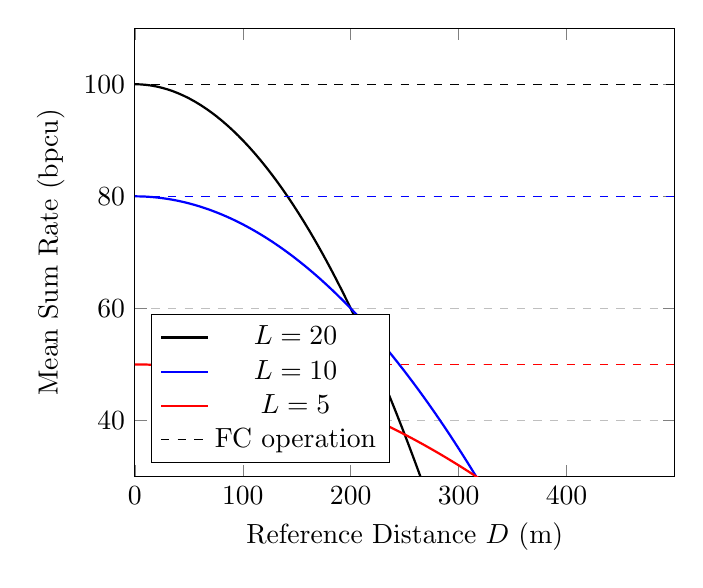
\begin{tikzpicture}
        \begin{axis}[
            xlabel={Reference Distance $D$ (m)},
            ylabel={Mean Sum Rate (bpcu)},
            xmin=0, xmax=500,
            ymin=30, ymax=110,
            xtick={0,100,200,300,400},
            ytick={40,60,80,100},
            legend pos=south west,
            ymajorgrids=true,
            grid style=dashed,
        ]
        
        % Plot data for L = 20
        \addplot[
            domain=0:500, 
            samples=100, 
            color=black,
            thick,
        ] {100 - 0.001 * x^2};
        \addlegendentry{$L = 20$}
        
        % Plot data for L = 10
        \addplot[
            domain=0:500, 
            samples=100, 
            color=blue,
            thick,
        ] {80 - 0.0005 * x^2};
        \addlegendentry{$L = 10$}
        
        % Plot data for L = 5
        \addplot[
            domain=0:500, 
            samples=100, 
            color=red,
            thick,
        ] {50 - 0.0002 * x^2};
        \addlegendentry{$L = 5$}
        
        % Dashed lines for FC operation
        \addplot[
            domain=0:500, 
            samples=100, 
            color=black,
            dashed,
        ] {100};
        \addlegendentry{FC operation}
        
        \addplot[
            domain=0:500, 
            samples=100, 
            color=blue,
            dashed,
        ] {80};
        
        \addplot[
            domain=0:500, 
            samples=100, 
            color=red,
            dashed,
        ] {50};
        
        \end{axis}
    \end{tikzpicture}
    \caption{Sum rate of PCNC scheme with respect to the reference distance $D$. The dashed lines represent the sum rates of the FC operation. Parameters for the plot: $M=5$, $K=5$, $N=2$, and $d_{kc} = 2~\forall k,c$.}
    \label{fig:sum_rate_pcnc}
\end{figure}

\end{document}